\chapter{Resultados}
\label{chap:resultados}

Este capítulo presenta los resultados de la campaña principal ejecutada en
Finisterrae~III con Python~3.15.0b1t \emph{free-threaded}. La campaña mide tres
aspectos, la corrección funcional de los cinco benchmarks portados, el impacto
de los modos de ejecución de OMP4Py y la escalabilidad al aumentar el número de
hilos.

La campaña cubre CG, EP, FT, IS y MG, y cada clase se midió solo en las
configuraciones donde resultaba informativa.
La clase~S pasó por los cuatro modos, para validar todos los caminos de código.
En clase~W solo tiene sentido medir los modos compilados~2 y~3, porque los interpretados
ya no son representativos a ese tamaño. Y la clase~A se reservó al modo~3, porque
las clases menores dejan claro que sin tipado Cython no hay tiempos prácticos.
Todas las combinaciones usaron 1, 2, 4, 8, 16 y 32~hilos, con tres repeticiones
cada una.

La métrica principal es el tiempo NAS interno reportado por cada benchmark. Para
cada combinación se toma el mejor tiempo entre las repeticiones válidas. El
tiempo externo del proceso se conserva en los ficheros de resultados, pero no
se usa como métrica principal porque incluye arranque del intérprete,
importación, compilación y escritura de logs.

\begin{table}[htbp]
\centering
\small
\resizebox{\textwidth}{!}{%
\begin{tabular}{lrrrr}
\hline
Campaña & Ejecuciones & Correctas & Éxito & Alcance \\
\hline
Campaña principal Python~3.15t & 630 & 630 & 100\% & S: modos 0--3; W: modos 2--3; A: modo 3 \\
Comparación de versiones & 1440 & 1440 & 100\% & Python 3.13t, 3.14t y 3.15t; clases S y W; modos 2--3 \\
\hline
\end{tabular}
}
\caption{Cobertura de las campañas finales ejecutadas en Finisterrae~III.}
\label{tab:resultados-cobertura-global}
\end{table}


La Tabla~\ref{tab:resultados-cobertura-global} resume la cobertura final. Las
630 ejecuciones de la campaña principal terminaron con código de retorno cero y
verificación NAS \texttt{SUCCESSFUL}. Por tanto, el análisis de rendimiento se
realiza sobre implementaciones funcionalmente correctas.


\section{Efecto del modo de ejecución en clase S}
\label{sec:resultados-modos-s}

La clase~S permite comparar los cuatro modos de OMP4Py con bajo coste. El
modo~0 conserva la ejecución Python de referencia, el modo~1 aplica la
transformación OMP4Py sin compilar los kernels, el modo~2 genera código Cython
sin tipos explícitos y el modo~3 añade tipado Cython y \emph{memoryviews}.

\begin{table}[htbp]
\centering
\small
\begin{tabular}{lrrrrrr}
\hline
Benchmark & M0 (s) & M1 (s) & M2 (s) & M3 (s) & M0/M3 & M2/M3 \\
\hline
CG & 18.23 & 18.23 & 16.35 & 0.13 & 140.23$\times$ & 125.77$\times$ \\
EP & 51.97 & 50.45 & 42.32 & 1.44 & 36.09$\times$ & 29.39$\times$ \\
FT & 38.76 & 38.70 & 36.77 & 2.41 & 16.08$\times$ & 15.26$\times$ \\
IS & 0.33 & 0.33 & 0.30 & 0.00 & --- & --- \\
MG & 3.81 & 3.81 & 3.24 & 0.01 & 381.00$\times$ & 324.00$\times$ \\
\hline
\end{tabular}
\caption{Mejor tiempo NAS en clase~S con un hilo para los cuatro modos de ejecución en Python~3.15t.}
\label{tab:resultados-s-t1-modos}
\end{table}


\begin{figure}[htbp]
\centering
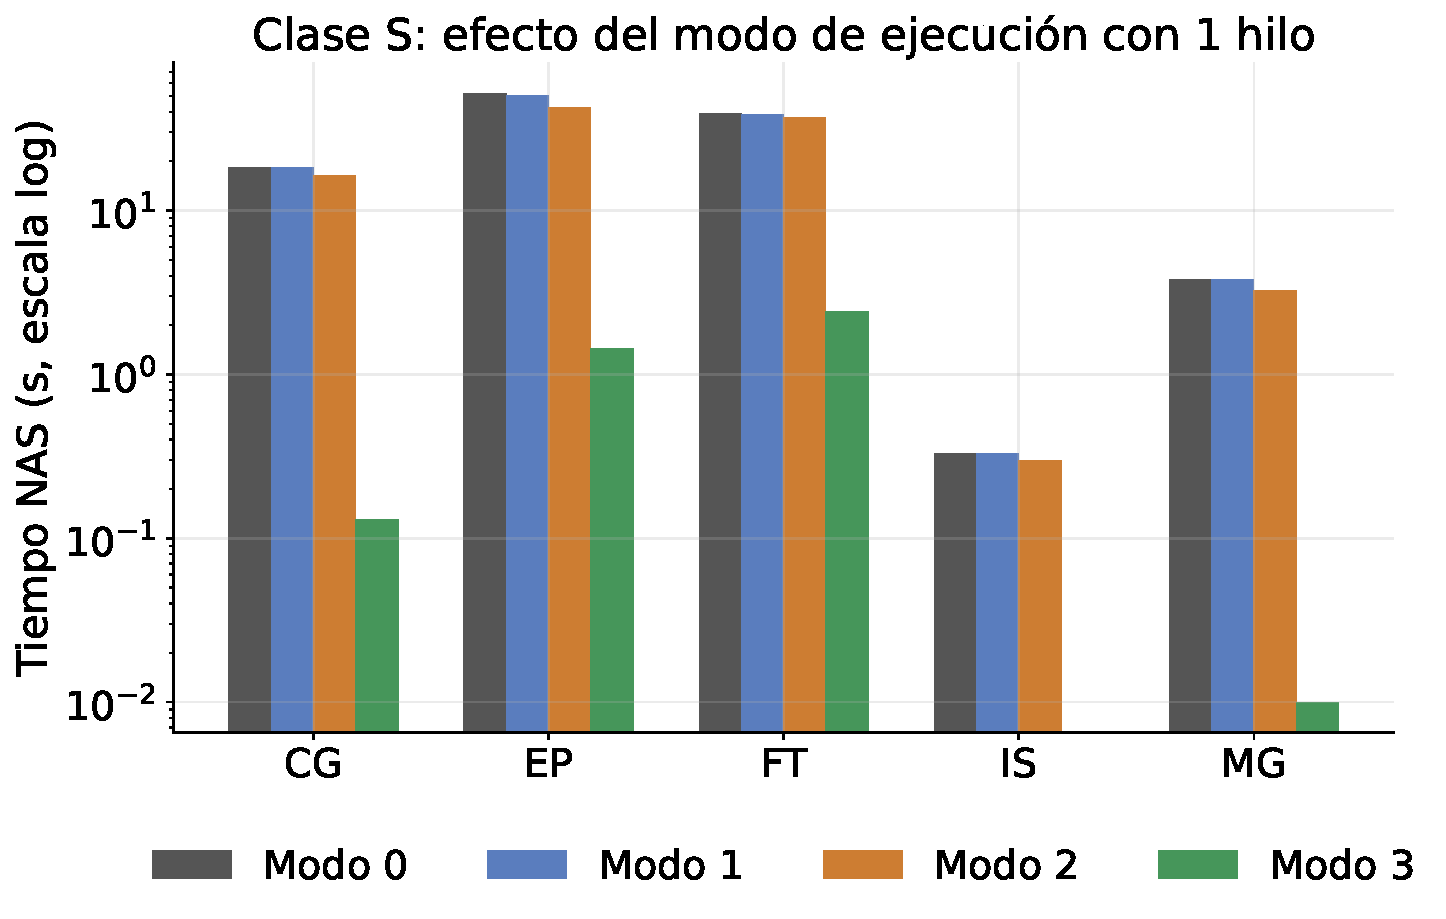
\includegraphics[width=\textwidth]{imagenes/resultados/clase_s_t1_modos}
\caption{Tiempo NAS con un hilo en clase~S para los cuatro modos de ejecución.
El eje vertical usa escala logarítmica.}
\label{fig:resultados-clase-s-modos}
\end{figure}

La Tabla~\ref{tab:resultados-s-t1-modos} y la
Figura~\ref{fig:resultados-clase-s-modos} muestran que el modo~3 obtiene el
menor tiempo con un hilo en todos los benchmarks. Frente al modo~0, los factores son
$140.23\times$ en CG, $36.09\times$ en EP, $16.08\times$ en FT y
$381.00\times$ en MG. IS aparece como 0.00~s en modo~3 porque el tiempo NAS se
imprime con dos decimales y la clase~S queda por debajo de esa resolución.

La diferencia entre modo~2 y modo~3 confirma que el cuello principal no es solo
la compilación, sino el tipado. En CG, el modo~2 tarda 16.35~s y el modo~3
0.13~s. En MG, el modo~2 tarda 3.24~s y el modo~3 0.01~s. EP y FT muestran el
mismo patrón con factores de $29.39\times$ y $15.26\times$. Sin anotaciones de
tipo, Cython conserva demasiada semántica de objetos Python dentro de los
bucles críticos. Con el modo~3, esos bucles pasan a ejecutarse como código
nativo efectivo.

Los modos~0 y~1 quedan prácticamente superpuestos con un hilo. La transformación
OMP4Py, por sí sola, no aporta rendimiento cuando no se combina con compilación
y tipado. En clase~S, su utilidad principal es validar que el código portado
mantiene caminos funcionales para todos los modos.


\section{Escalabilidad en clase S}
\label{sec:resultados-escalabilidad-s}

La clase~S no es la carga principal para extraer conclusiones de escalabilidad,
pero permite detectar qué kernels tienen suficiente trabajo incluso en tamaños
pequeños y qué modos introducen overhead dominante.

\begin{table}[htbp]
\centering
\small
\begin{tabular}{lrrrr}
\hline
Benchmark & M0 & M1 & M2 & M3 \\
\hline
CG & 0.96$\times$ & 0.96$\times$ & 2.34$\times$ & 0.15$\times$ \\
EP & 23.84$\times$ & 29.16$\times$ & 24.05$\times$ & 9.00$\times$ \\
FT & 4.00$\times$ & 4.05$\times$ & 4.79$\times$ & 9.64$\times$ \\
IS & 1.00$\times$ & 1.00$\times$ & 1.25$\times$ & --- \\
MG & 2.10$\times$ & 2.23$\times$ & 8.53$\times$ & 0.05$\times$ \\
\hline
\end{tabular}
\caption{Speedup a 32 hilos respecto a 1 hilo en clase~S para cada modo de Python~3.15t.}
\label{tab:resultados-s-speedup32-modos}
\end{table}


\begin{figure}[htbp]
\centering
\begin{subfigure}[t]{0.49\textwidth}
  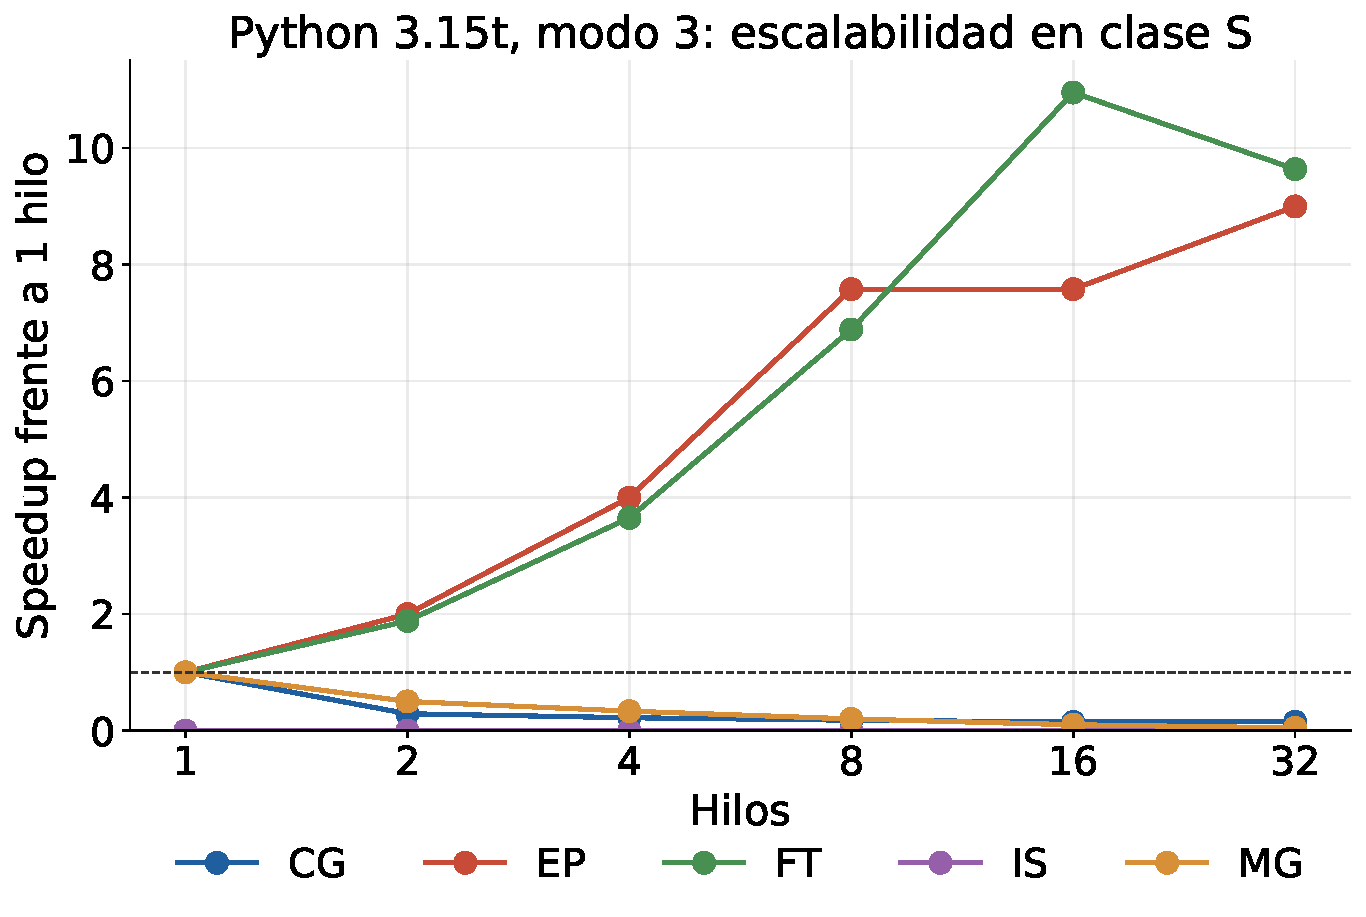
\includegraphics[width=\textwidth]{imagenes/resultados/mode3_speedup_clase_s}
  \caption{Speedup. La línea discontinua marca el umbral de speedup~1.}
  \label{fig:resultados-speedup-s}
\end{subfigure}\hfill
\begin{subfigure}[t]{0.49\textwidth}
  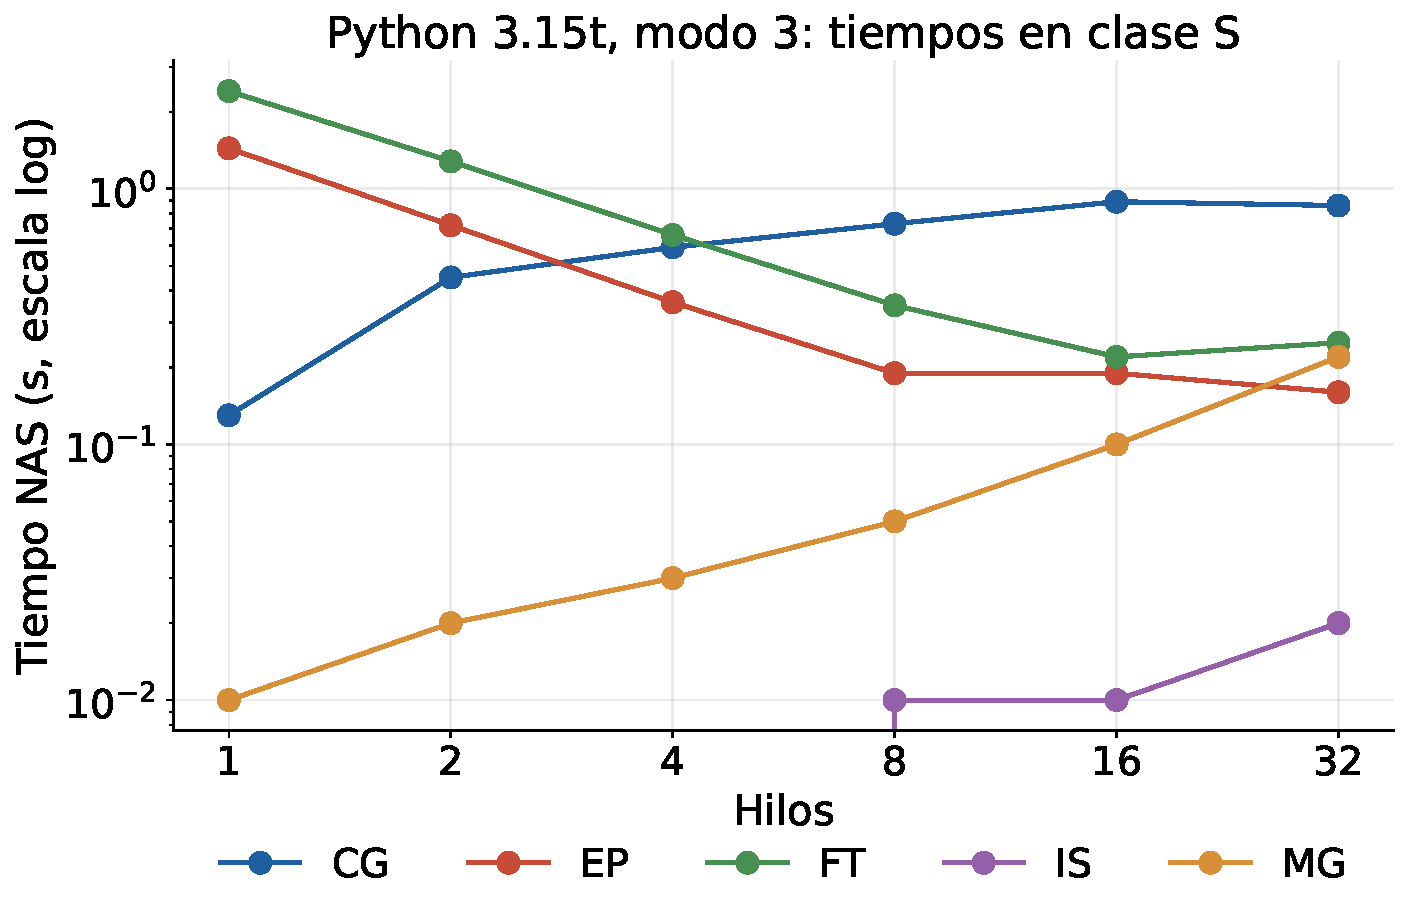
\includegraphics[width=\textwidth]{imagenes/resultados/mode3_tiempo_clase_s}
  \caption{Tiempo NAS por número de hilos.}
  \label{fig:resultados-tiempo-s}
\end{subfigure}
\caption{Clase~S, modo~3, Python~3.15t. Speedup y tiempo NAS por número de
hilos. Cada línea corresponde a un benchmark.}
\label{fig:resultados-clase-s-escalabilidad}
\end{figure}

La Tabla~\ref{tab:resultados-s-speedup32-modos} muestra que EP y FT ya obtienen
speedups apreciables a 32~hilos en clase~S. En modo~3, EP alcanza
$9.00\times$ y FT $9.64\times$. En EP, los modos~0,~1 y~2 también muestran
speedups altos, señal de que el kernel dispone de trabajo paralelo suficiente
incluso en la clase pequeña.

El caso de EP en los modos interpretados merece una lectura propia. En modo~1,
EP alcanza $29.16\times$ a 32~hilos, una aceleración casi lineal sobre código
Python interpretado. Este resultado es la evidencia más directa de la campaña
de que el intérprete \emph{free-threaded} cumple su objetivo. Sin el GIL, los
hilos Python ejecutan trabajo en paralelo real sin necesidad de compilación
alguna. Que el speedup relativo del modo~3 sea menor ($9.00\times$) no
contradice esa lectura. El tipado acelera el cómputo pero no la sincronización,
por lo que la fracción de espera pesa más cuanto más rápido es el kernel. La
comparación en tiempo absoluto mantiene, no obstante, la conclusión práctica.
El modo~3 con un hilo (1.44~s) ya es más rápido que el modo~1 con 32~hilos
(aproximadamente 1.7~s), de modo que la escalabilidad casi ideal del modo
interpretado tiene valor diagnóstico, no práctico.

El comportamiento no es uniforme. CG y MG empeoran en modo~3, con
$0.15\times$ y $0.05\times$ respectivamente. IS no permite calcular un speedup
fiable en modo~3 porque el tiempo base aparece redondeado a 0.00~s. La clase~S
confirma, por tanto, una división que se mantiene en clases mayores. EP y FT
son los candidatos naturales a escalar, mientras que CG, IS y MG están más
condicionados por sincronización, granularidad o accesos irregulares.

La lectura metodológica es que la clase~S sirve para validar todos los caminos y
para observar tendencias iniciales, pero las conclusiones prácticas deben
apoyarse en W y A. En tamaños tan pequeños, pequeñas diferencias de tiempo o de
redondeo pueden afectar mucho a los cocientes.


\section{Modos compilados en clase W}
\label{sec:resultados-clase-w}

La clase~W aumenta el tamaño del problema y restringe la comparación a los
modos~2 y~3. Esta decisión evita dedicar recursos a modos interpretados que ya
son varios órdenes de magnitud más lentos en clase~S.

\begin{table}[htbp]
\centering
\small
\begin{tabular}{lrrr}
\hline
Benchmark & M2 (s) & M3 (s) & M2/M3 \\
\hline
CG & 105.6 & 0.78 & 135.42$\times$ \\
EP & 84.53 & 2.87 & 29.45$\times$ \\
FT & 80.07 & 5.04 & 15.89$\times$ \\
IS & 5.54 & 0.03 & 184.67$\times$ \\
MG & 198.2 & 0.45 & 440.51$\times$ \\
\hline
\end{tabular}
\caption{Mejor tiempo NAS en clase~W con un hilo para los modos compilados de Python~3.15t.}
\label{tab:resultados-w-t1-modos}
\end{table}


La Tabla~\ref{tab:resultados-w-t1-modos} mantiene la misma conclusión de clase~S.
El modo~3 es la única configuración con tiempos prácticos. Con un hilo, el modo~2 tarda 105.6~s en CG frente a 0.78~s en
modo~3. En MG la diferencia es de 198.2~s frente a 0.45~s. EP y FT mantienen
factores de mejora cercanos a $29.45\times$ y $15.89\times$, e IS mejora de
5.54~s a 0.03~s.

\begin{table}[htbp]
\centering
\small
\begin{tabular}{lrr}
\hline
Benchmark & M2 & M3 \\
\hline
CG & 7.77$\times$ & 0.14$\times$ \\
EP & 26.09$\times$ & 9.90$\times$ \\
FT & 4.37$\times$ & 8.00$\times$ \\
IS & 0.81$\times$ & 0.43$\times$ \\
MG & 23.68$\times$ & 0.57$\times$ \\
\hline
\end{tabular}
\caption{Speedup a 32~hilos respecto a 1~hilo en clase~W para los modos compilados de Python~3.15t.}
\label{tab:resultados-w-speedup32-modos}
\end{table}



\begin{figure}[htbp]
\centering
\begin{subfigure}[t]{0.49\textwidth}
  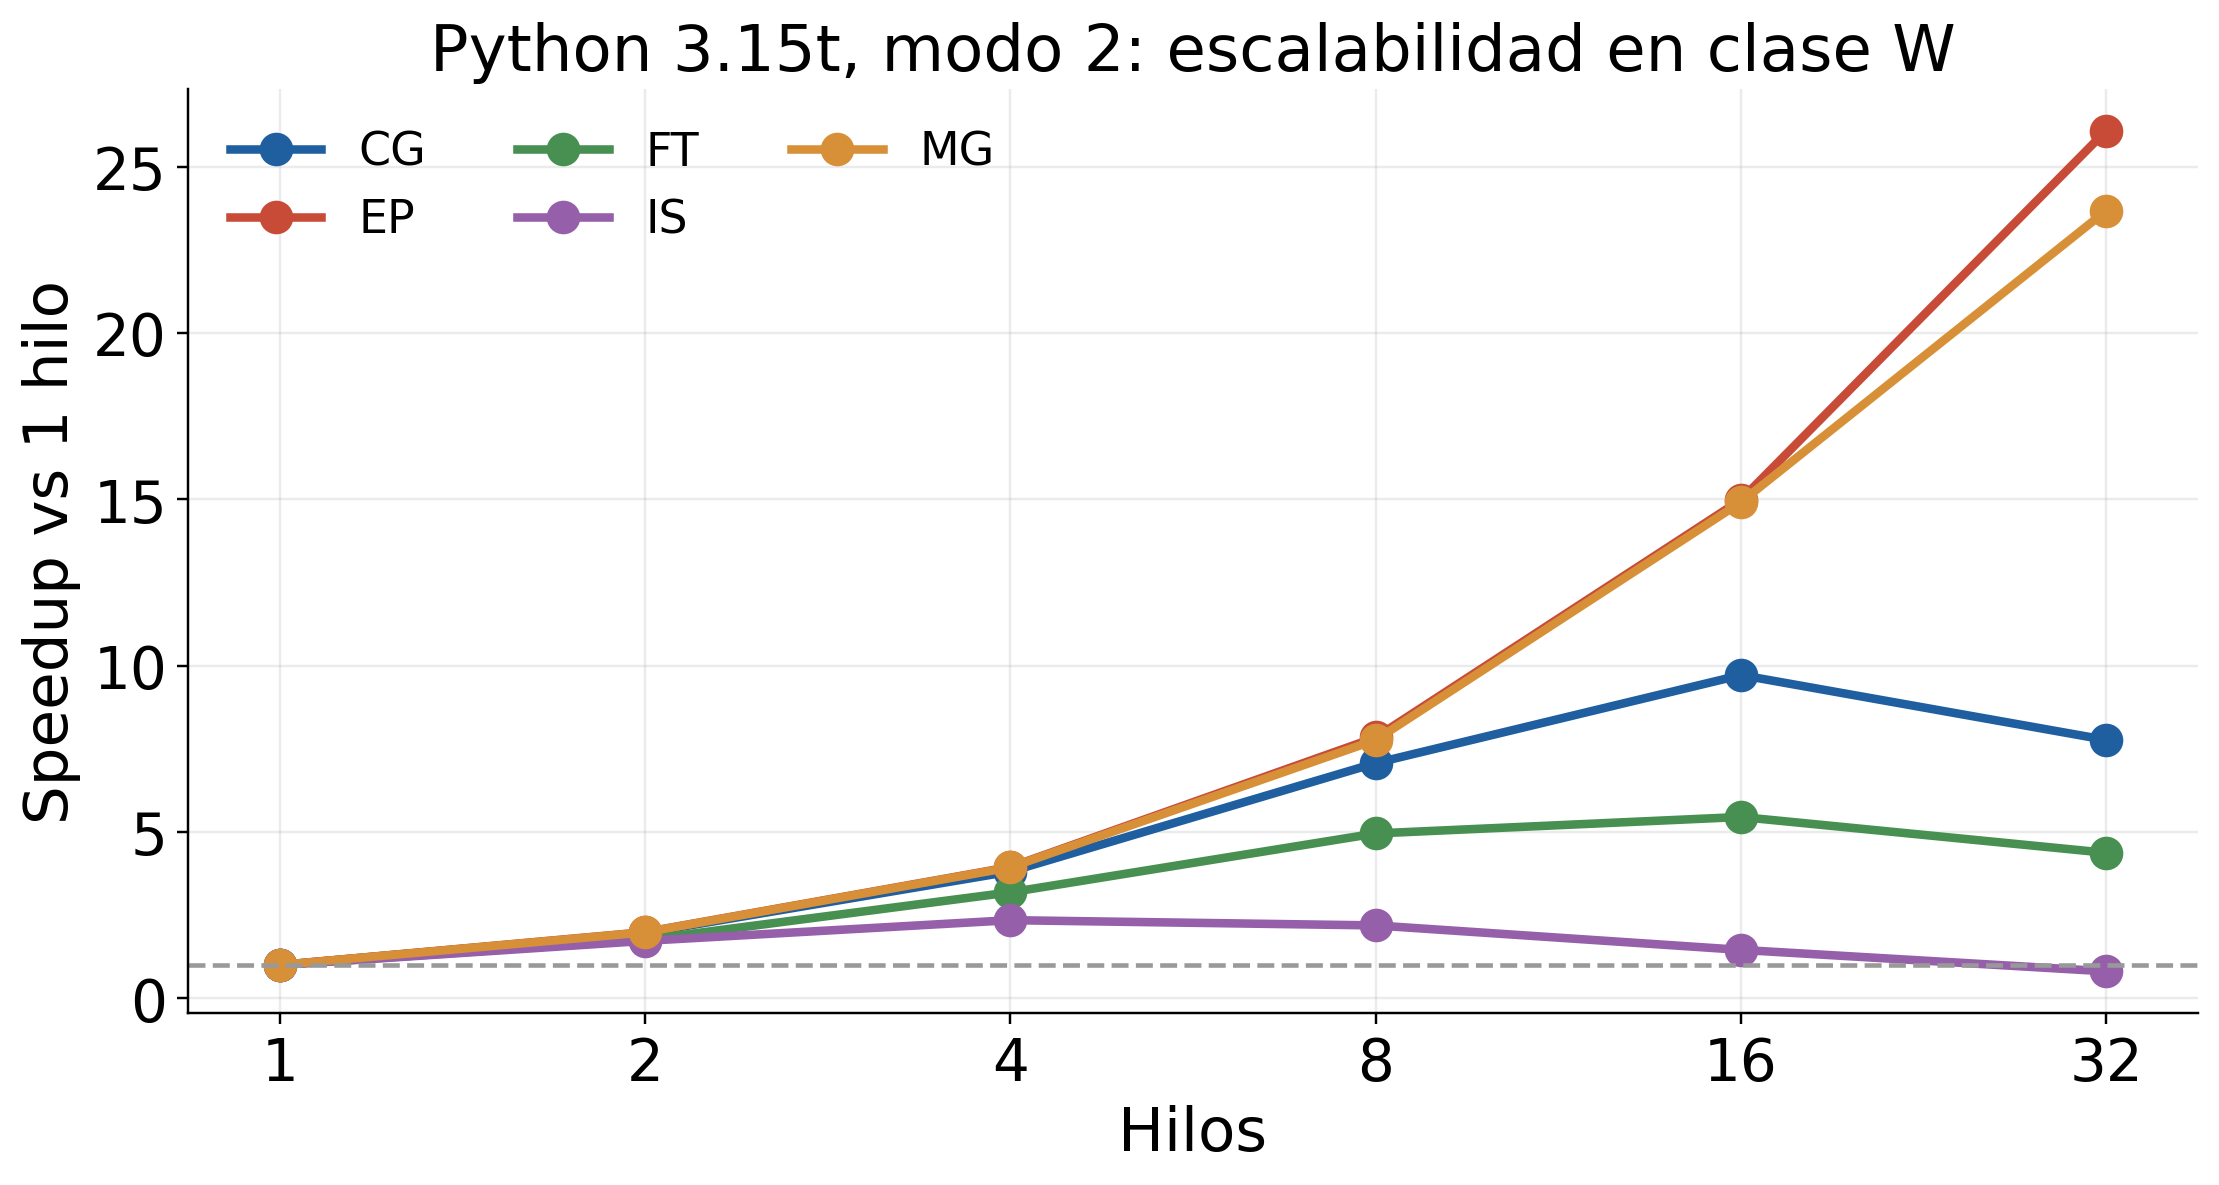
\includegraphics[width=\textwidth]{imagenes/resultados/mode2_speedup_clase_w}
  \caption{Speedup.}
  \label{fig:resultados-speedup-w-m2}
\end{subfigure}\hfill
\begin{subfigure}[t]{0.49\textwidth}
  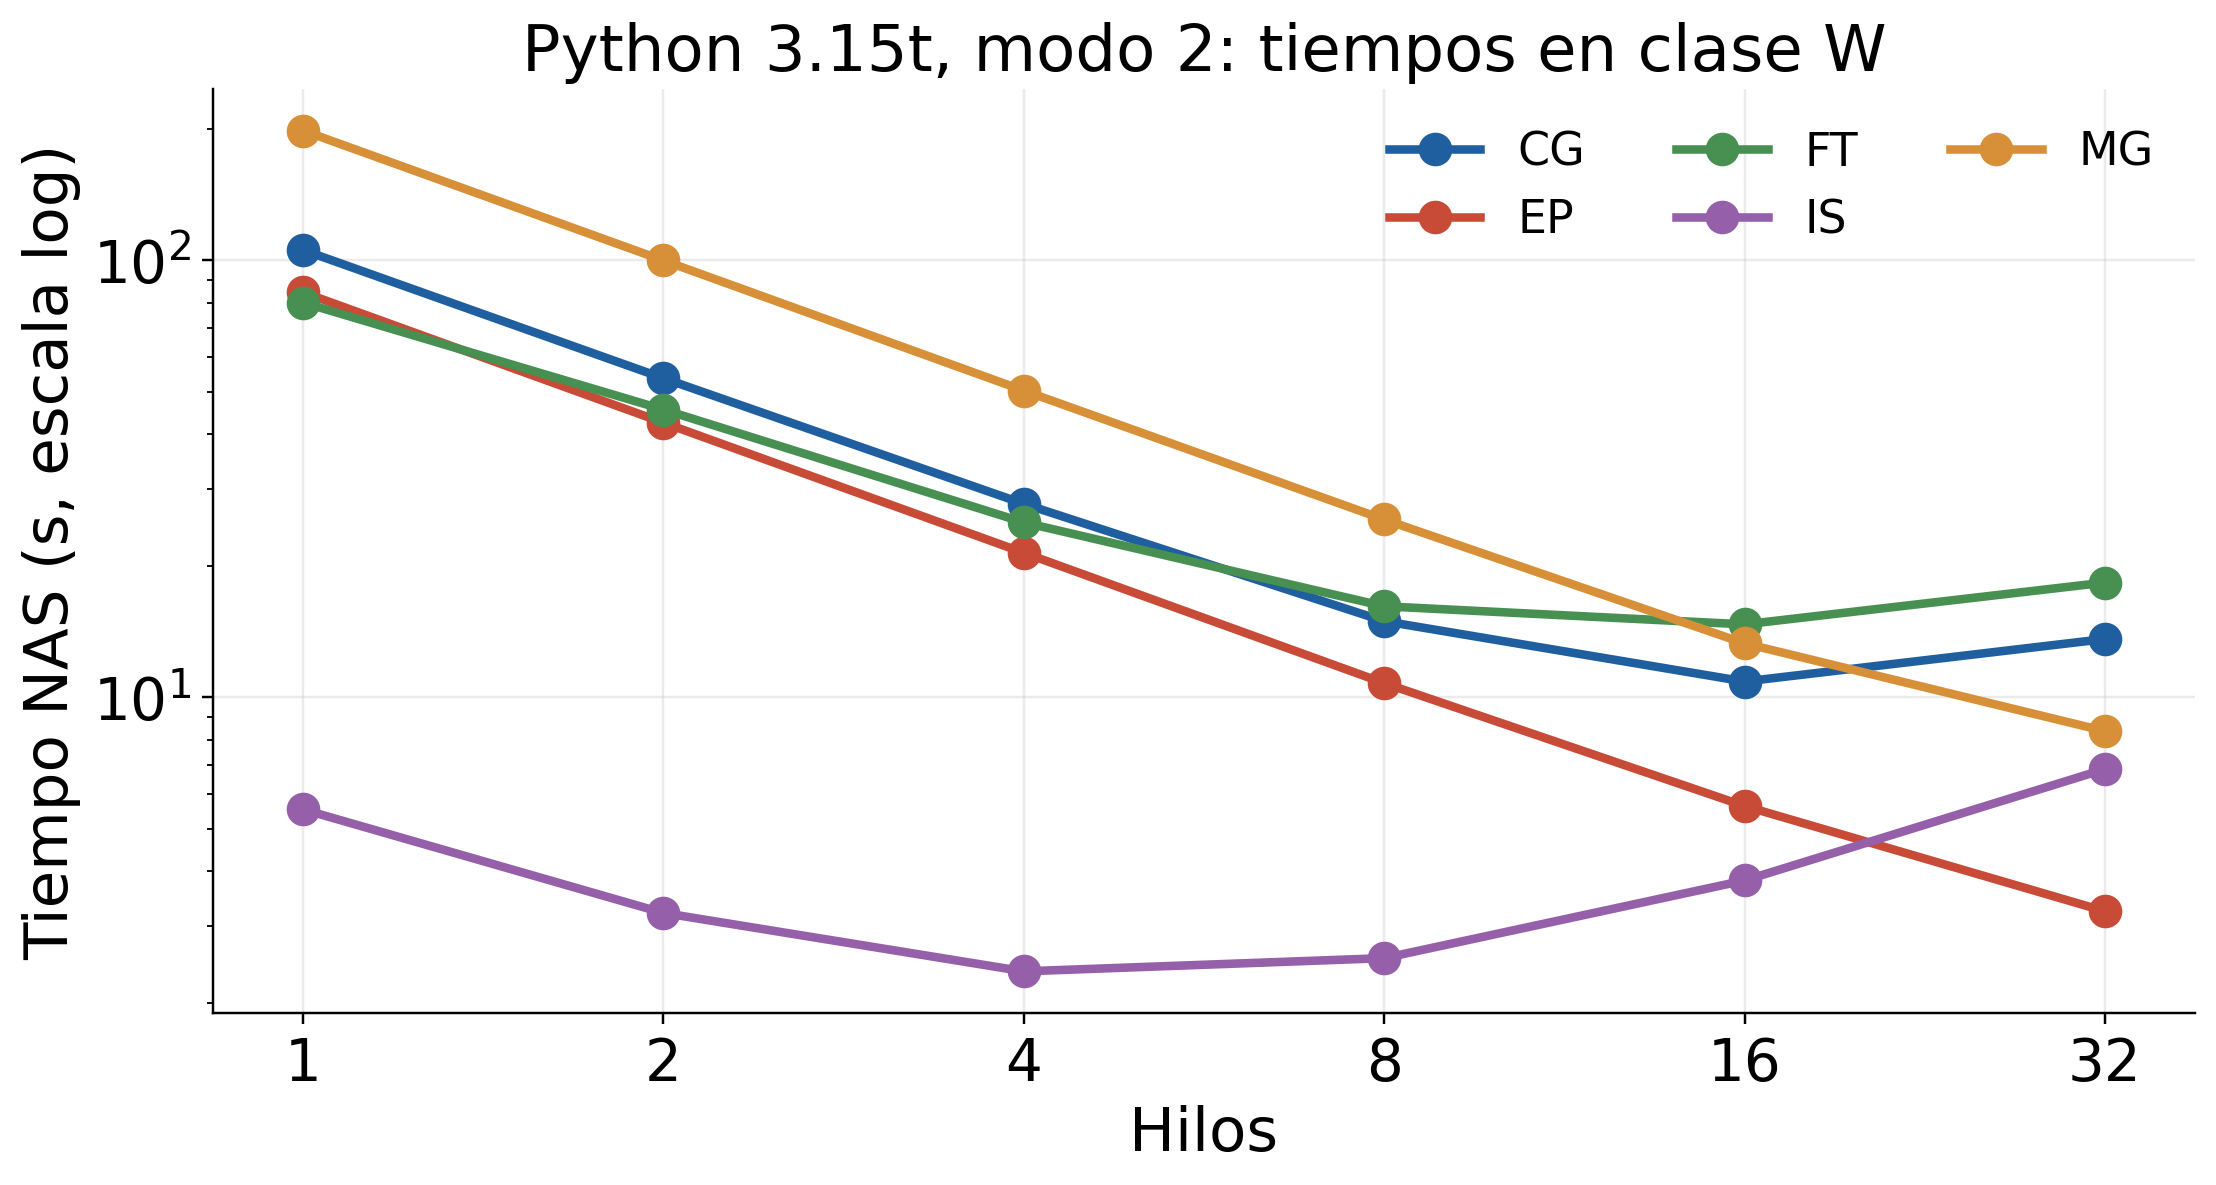
\includegraphics[width=\textwidth]{imagenes/resultados/mode2_tiempo_clase_w}
  \caption{Tiempo NAS por número de hilos.}
  \label{fig:resultados-tiempo-w-m2}
\end{subfigure}
\caption{Clase~W, modo~2, Python~3.15t. Speedup y tiempo NAS por número de
hilos.}
\label{fig:resultados-clase-w-mode2}
\end{figure}

\begin{figure}[htbp]
\centering
\begin{subfigure}[t]{0.49\textwidth}
  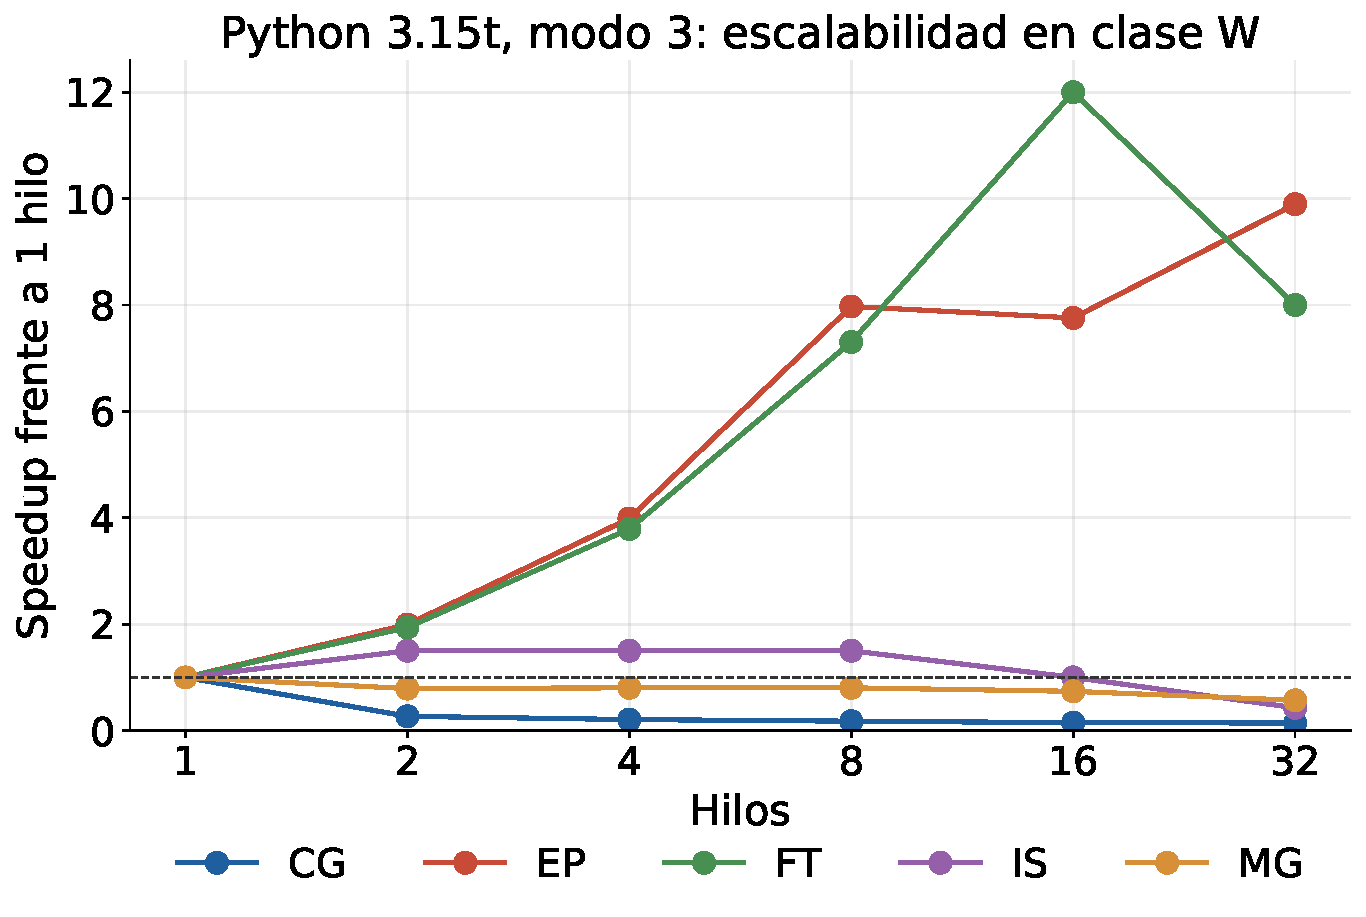
\includegraphics[width=\textwidth]{imagenes/resultados/mode3_speedup_clase_w}
  \caption{Speedup.}
  \label{fig:resultados-speedup-w}
\end{subfigure}\hfill
\begin{subfigure}[t]{0.49\textwidth}
  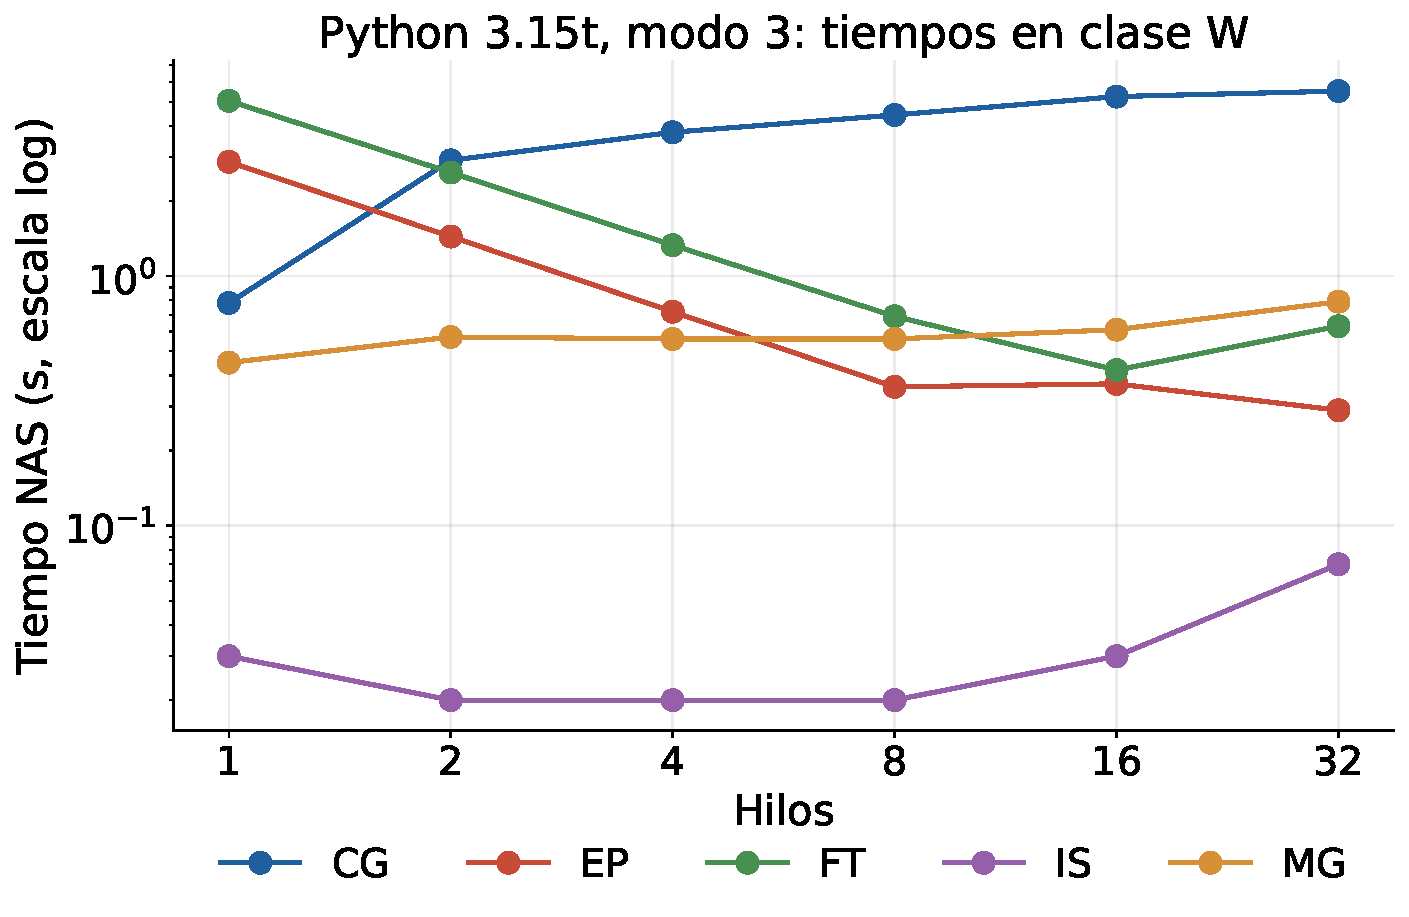
\includegraphics[width=\textwidth]{imagenes/resultados/mode3_tiempo_clase_w}
  \caption{Tiempo NAS por número de hilos.}
  \label{fig:resultados-tiempo-w}
\end{subfigure}
\caption{Clase~W, modo~3, Python~3.15t. Speedup y tiempo NAS por número de
hilos. Cada línea corresponde a un benchmark.}
\label{fig:resultados-clase-w-escalabilidad}
\end{figure}

La escalabilidad en clase~W separa los benchmarks en dos grupos. En modo~3, EP
alcanza su mejor tiempo con 32~hilos, bajando de 2.87~s a 0.29~s
($9.90\times$), y FT llega a $8.00\times$. FT obtiene su mejor punto con
16~hilos, donde baja de 5.04~s a 0.42~s, equivalente a $12.00\times$.

CG, IS y MG no escalan en modo~3. CG cae a $0.14\times$, IS a $0.43\times$ y
MG a $0.57\times$ a 32~hilos. El modo~2 sí muestra speedups altos en varios de
estos casos, por ejemplo $7.77\times$ en CG y $23.68\times$ en MG
(Figura~\ref{fig:resultados-clase-w-mode2}), pero sus tiempos absolutos siguen
siendo muy superiores a los del modo~3 con un hilo. El speedup aislado, por sí
solo, no basta para escoger configuración. Un modo puede escalar mejor en
términos relativos y seguir siendo peor en tiempo absoluto.



\section{Evaluación de escalabilidad en clase A}
\label{sec:resultados-clase-a}

La clase~A es la carga de mayor tamaño de la campaña principal. Se ejecutó solo
en modo~3 porque es la única configuración que produce tiempos prácticos en las
clases anteriores.

\begin{table}[htbp]
\centering
\small
\begin{tabular}{lrrrrrr}
\hline
Benchmark & 1 & 2 & 4 & 8 & 16 & 32 \\
\hline
CG & 2.76 & 10.29 & 14.35 & 15.98 & 18.91 & 21.17 \\
EP & 22.99 & 11.48 & 5.75 & 2.88 & 2.90 & 2.19 \\
FT & 58.63 & 30.05 & 15.26 & 7.70 & 3.99 & 4.18 \\
IS & 0.36 & 0.21 & 0.15 & 0.18 & 0.24 & 0.44 \\
MG & 3.57 & 4.34 & 4.14 & 3.96 & 3.79 & 4.56 \\
\hline
\end{tabular}
\caption{Mejor tiempo NAS en clase~A, modo~3, Python~3.15t.}
\label{tab:resultados-a-mode3-tiempos}
\end{table}


\begin{table}[htbp]
\centering
\small
\begin{tabular}{lrrrrrr}
\hline
Benchmark & 1 & 2 & 4 & 8 & 16 & 32 \\
\hline
CG & 1.00$\times$ & 0.27$\times$ & 0.19$\times$ & 0.17$\times$ & 0.15$\times$ & 0.13$\times$ \\
EP & 1.00$\times$ & 2.00$\times$ & 4.00$\times$ & 7.98$\times$ & 7.93$\times$ & 10.50$\times$ \\
FT & 1.00$\times$ & 1.95$\times$ & 3.84$\times$ & 7.61$\times$ & 14.69$\times$ & 14.03$\times$ \\
IS & 1.00$\times$ & 1.71$\times$ & 2.40$\times$ & 2.00$\times$ & 1.50$\times$ & 0.82$\times$ \\
MG & 1.00$\times$ & 0.82$\times$ & 0.86$\times$ & 0.90$\times$ & 0.94$\times$ & 0.78$\times$ \\
\hline
\end{tabular}
\caption{Speedup por número de hilos en clase~A, modo~3, Python~3.15t.}
\label{tab:resultados-a-mode3-speedups}
\end{table}


\begin{figure}[htbp]
\centering
\begin{subfigure}[t]{0.49\textwidth}
  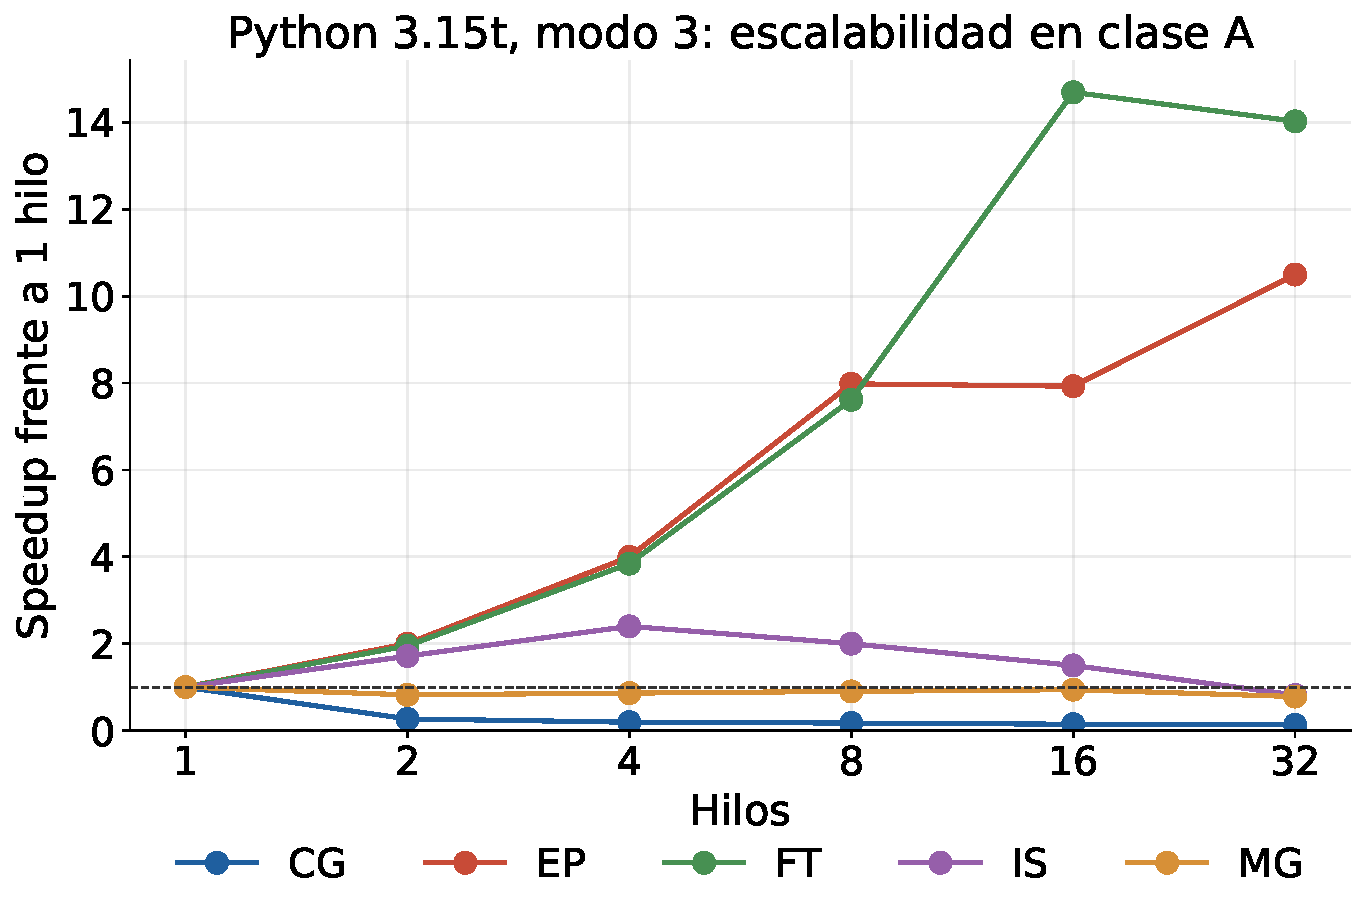
\includegraphics[width=\textwidth]{imagenes/resultados/mode3_speedup_clase_a}
  \caption{Speedup.}
  \label{fig:resultados-speedup-a}
\end{subfigure}\hfill
\begin{subfigure}[t]{0.49\textwidth}
  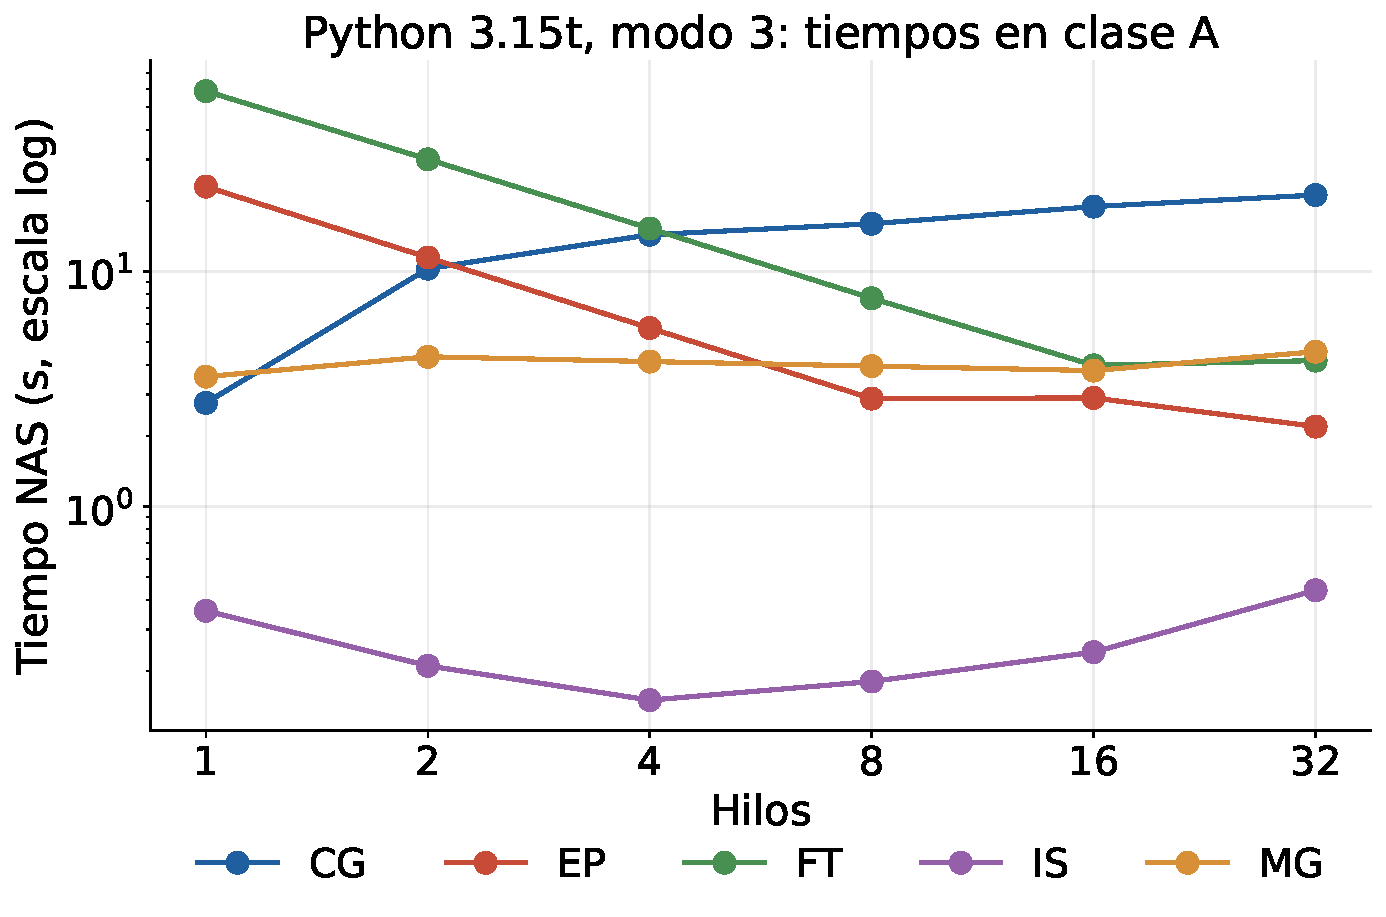
\includegraphics[width=\textwidth]{imagenes/resultados/mode3_tiempo_clase_a}
  \caption{Tiempo NAS por número de hilos.}
  \label{fig:resultados-tiempo-a}
\end{subfigure}
\caption{Clase~A, modo~3, Python~3.15t. Speedup y tiempo NAS por número de
hilos. Cada línea corresponde a un benchmark.}
\label{fig:resultados-clase-a-escalabilidad}
\end{figure}

Los resultados de clase~A son los más representativos para valorar el port en
cargas grandes. EP baja de 22.99~s con un hilo a 2.19~s con 32~hilos, lo que
supone $10.50\times$. FT baja de 58.63~s a 4.18~s con 32~hilos
($14.03\times$), y su mejor punto está en 16~hilos con 3.99~s
($14.69\times$). Estos dos benchmarks muestran que Python~3.15t, OMP4Py y el
código Cython tipado pueden producir escalabilidad real cuando el kernel ofrece
trabajo paralelo suficiente y una estructura adecuada.

IS obtiene una mejora moderada con pocos hilos. Pasa de 0.36~s a 0.15~s con
4~hilos, equivalente a $2.40\times$. Sin embargo, la curva empeora después y a
32~hilos cae a $0.82\times$. El tamaño de clase~A permite amortizar parte del
coste inicial, pero no sostiene la eficiencia al aumentar la concurrencia.

CG y MG no escalan en clase~A. CG empeora desde 2.76~s con un hilo hasta
21.17~s con 32~hilos. MG sube de 3.57~s a 4.56~s. Aquí se mantiene la lectura de
resultados. Más hilos no se traducen en menos tiempo. El
Capítulo~\ref{chap:profiling} analiza después las causas de esa degradación.


\section{Síntesis global del modo 3}
\label{sec:resultados-sintesis-mode3}

Como el modo~3 es el único que produce tiempos competitivos en todas las
clases, la síntesis global se centra en esa configuración.

\begin{table}[htbp]
\centering
\small
\resizebox{\textwidth}{!}{%
\begin{tabular}{llrrrrrrr}
\hline
Clase & Bench. & Mejor hilo & Mejor tiempo (s) & T1 (s) & Speedup ópt. & T32 (s) & Speedup32 & Mop/s32 \\
\hline
S & CG & 1 & 0.13 & 0.13 & 1.00$\times$ & 0.86 & 0.15$\times$ & 77.9 \\
S & EP & 32 & 0.16 & 1.44 & 9.00$\times$ & 0.16 & 9.00$\times$ & 213 \\
S & FT & 16 & 0.22 & 2.41 & 10.95$\times$ & 0.25 & 9.64$\times$ & 702 \\
S & IS & 1 & 0.00 & 0.00 & --- & 0.02 & 0.00$\times$ & 27.7 \\
S & MG & 1 & 0.01 & 0.01 & 1.00$\times$ & 0.22 & 0.05$\times$ & 33.9 \\
W & CG & 1 & 0.78 & 0.78 & 1.00$\times$ & 5.51 & 0.14$\times$ & 76.3 \\
W & EP & 32 & 0.29 & 2.87 & 9.90$\times$ & 0.29 & 9.90$\times$ & 229 \\
W & FT & 16 & 0.42 & 5.04 & 12.00$\times$ & 0.63 & 8.00$\times$ & 592 \\
W & IS & 2 & 0.02 & 0.03 & 1.50$\times$ & 0.07 & 0.43$\times$ & 158 \\
W & MG & 1 & 0.45 & 0.45 & 1.00$\times$ & 0.79 & 0.57$\times$ & 618 \\
A & CG & 1 & 2.76 & 2.76 & 1.00$\times$ & 21.17 & 0.13$\times$ & 70.7 \\
A & EP & 32 & 2.19 & 22.99 & 10.50$\times$ & 2.19 & 10.50$\times$ & 245 \\
A & FT & 16 & 3.99 & 58.63 & 14.69$\times$ & 4.18 & 14.03$\times$ & 1706 \\
A & IS & 4 & 0.15 & 0.36 & 2.40$\times$ & 0.44 & 0.82$\times$ & 191 \\
A & MG & 1 & 3.57 & 3.57 & 1.00$\times$ & 4.56 & 0.78$\times$ & 854 \\
\hline
\end{tabular}
}
\caption{Mejor número de hilos, speedup y rendimiento (Mop/s) a 32~hilos en
modo~3, Python~3.15t.}
\label{tab:resultados-mode3-optimos}
\end{table}


La Tabla~\ref{tab:resultados-mode3-optimos} resume el mejor número de hilos en
cada combinación y recoge además los tiempos y los Mop/s a 32~hilos, mientras
que la Figura~\ref{fig:resultados-speedup32-global} muestra de forma compacta
qué combinaciones escalan a 32~hilos y cuáles retroceden. EP alcanza su mejor
punto en 32~hilos en las tres clases, con $9.00\times$ en S, $9.90\times$ en W y
$10.50\times$ en A. FT alcanza su mejor punto en 16~hilos, con $10.95\times$ en
S, $12.00\times$ en W y $14.69\times$ en A. IS solo muestra una mejora clara en
A hasta 4~hilos. CG y MG mantienen el óptimo en un hilo en las tres clases.

Los Mop/s a 32~hilos refuerzan esa lectura. FT clase~A alcanza 1706~Mop/s y EP
clase~A 245~Mop/s con speedups superiores a $10\times$. En MG, en cambio, la
cifra de 854~Mop/s a 32~hilos no implica escalabilidad, porque el tiempo empeora
frente a un hilo. De ahí que el análisis combine siempre tiempo absoluto,
speedup y Mop/s.

\begin{figure}[htbp]
\centering
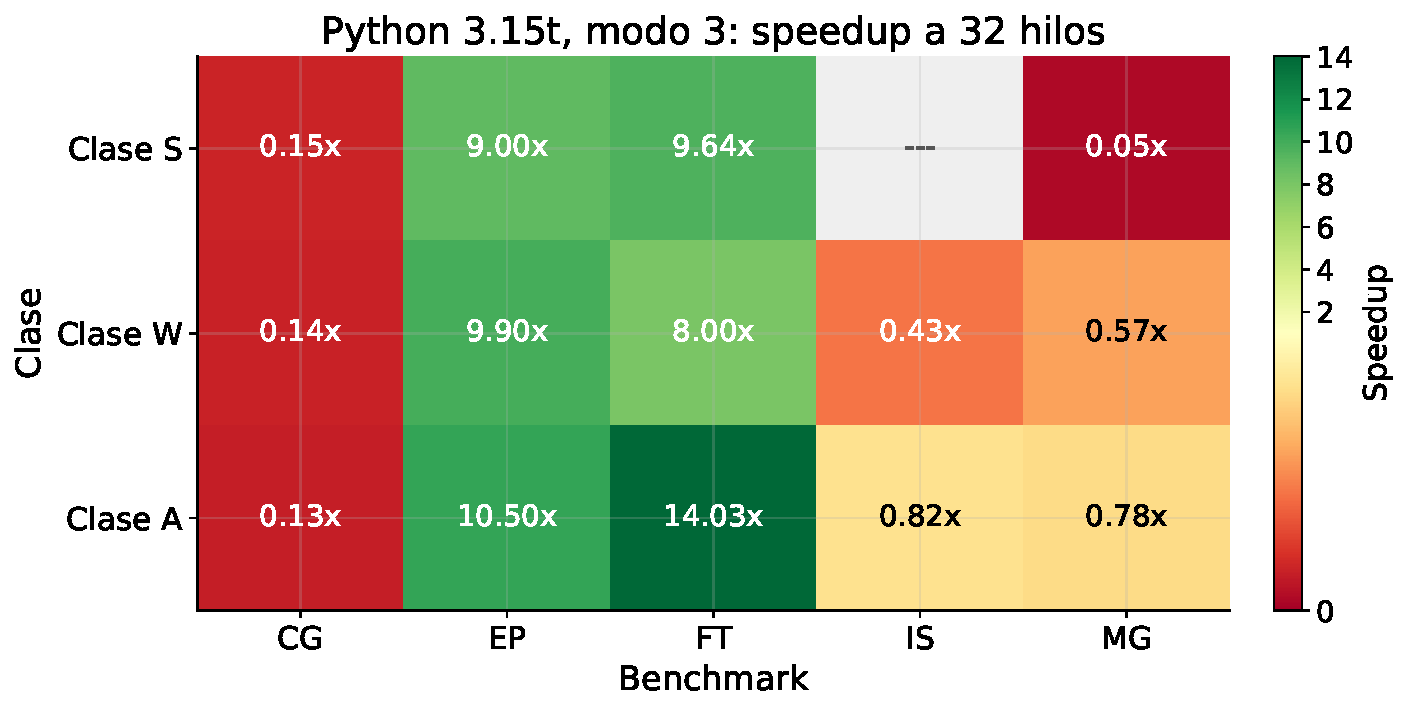
\includegraphics[width=\textwidth]{imagenes/resultados/mode3_speedup32_global}
\caption{Mapa de calor del speedup a 32~hilos en modo~3, Python~3.15t, para
las clases~S, W y A.}
\label{fig:resultados-speedup32-global}
\end{figure}


\section{Curvas por benchmark}
\label{sec:resultados-curvas-benchmark}

La Figura~\ref{fig:resultados-benchmark-clases} reorganiza la misma información
por benchmark. En cada panel, cada línea corresponde a una clase de problema.
Esta vista facilita comparar si el aumento de tamaño cambia la forma de la curva
de escalabilidad.

\begin{figure}[htbp]
\centering
\begin{subfigure}[t]{0.49\textwidth}
  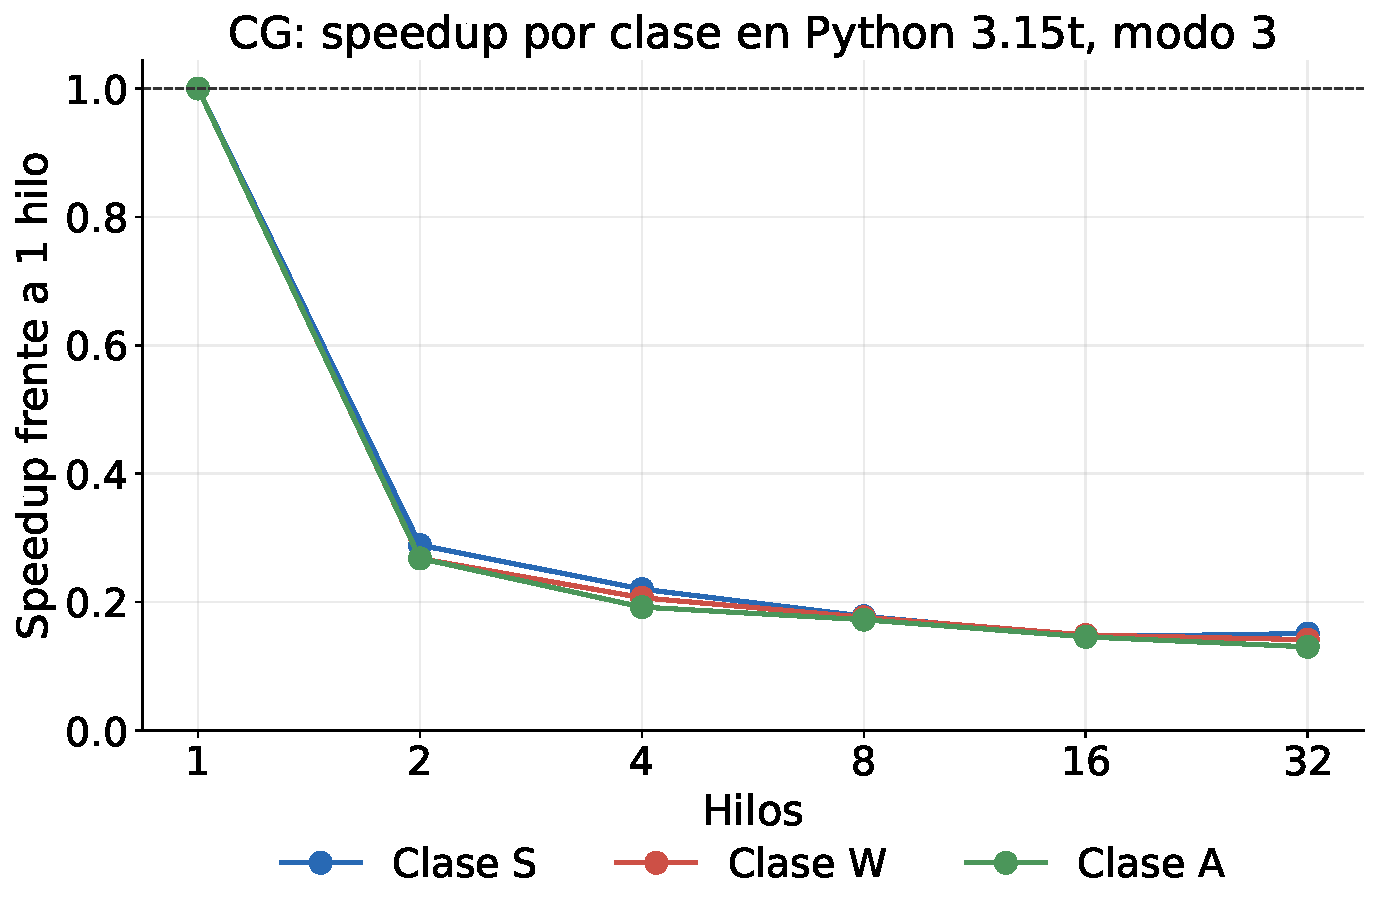
\includegraphics[width=\textwidth]{imagenes/resultados/benchmark_cg_speedup_clases}
  \caption{CG.}
  \label{fig:resultados-cg-clases}
\end{subfigure}\hfill
\begin{subfigure}[t]{0.49\textwidth}
  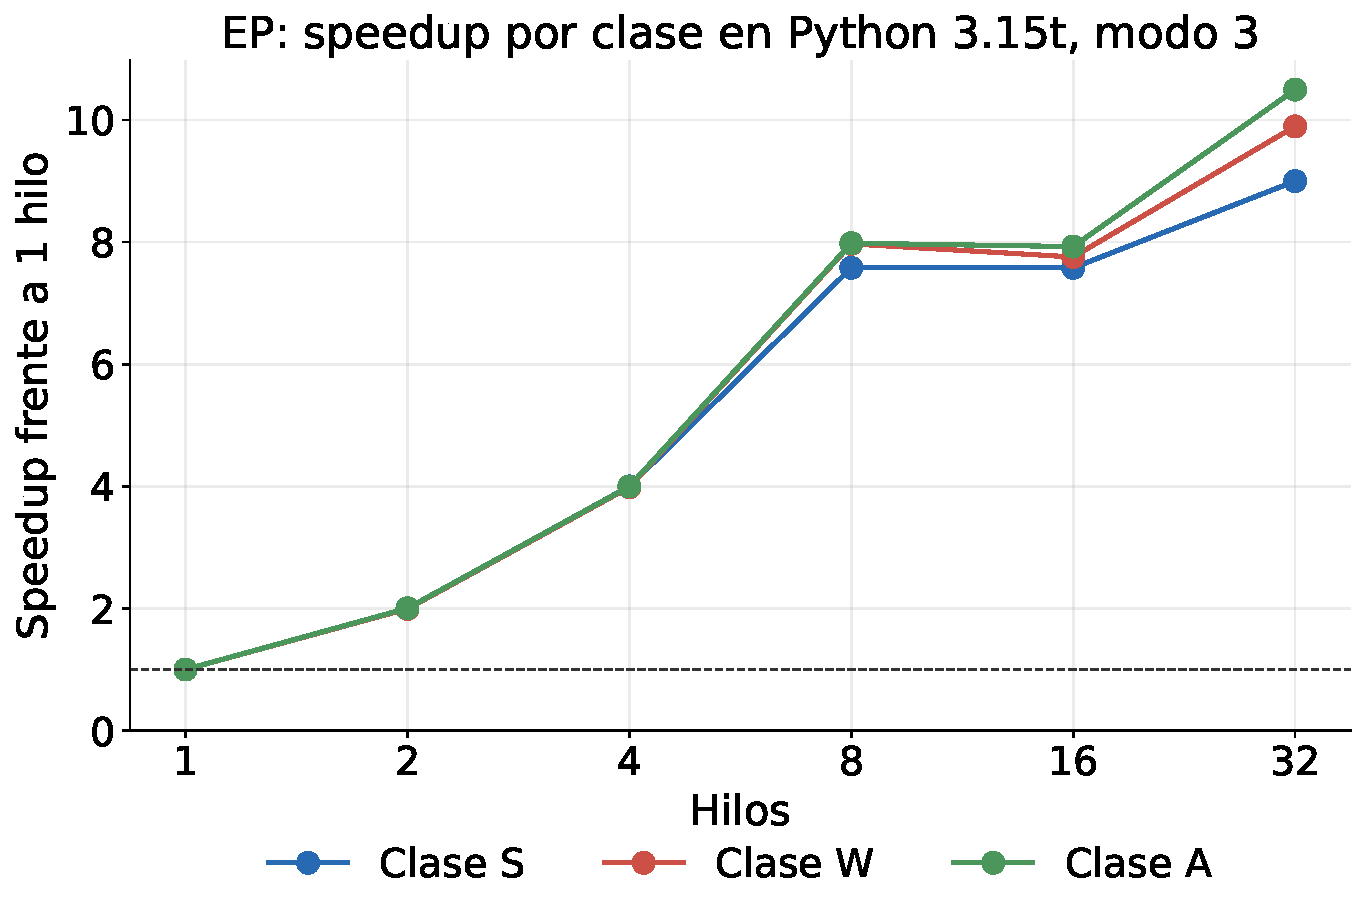
\includegraphics[width=\textwidth]{imagenes/resultados/benchmark_ep_speedup_clases}
  \caption{EP.}
  \label{fig:resultados-ep-clases}
\end{subfigure}

\vspace{0.8em}
\begin{subfigure}[t]{0.49\textwidth}
  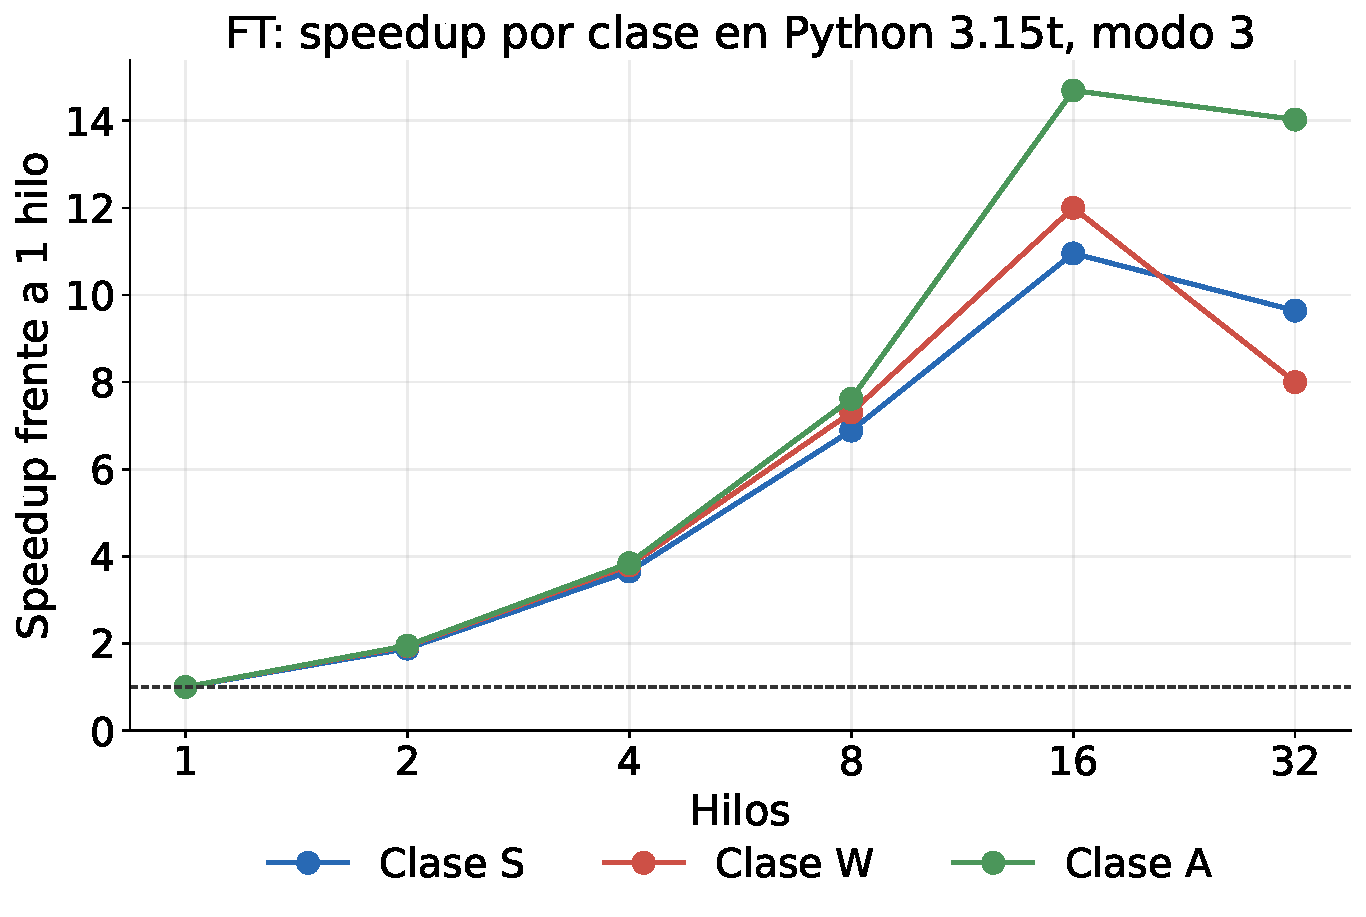
\includegraphics[width=\textwidth]{imagenes/resultados/benchmark_ft_speedup_clases}
  \caption{FT.}
  \label{fig:resultados-ft-clases}
\end{subfigure}\hfill
\begin{subfigure}[t]{0.49\textwidth}
  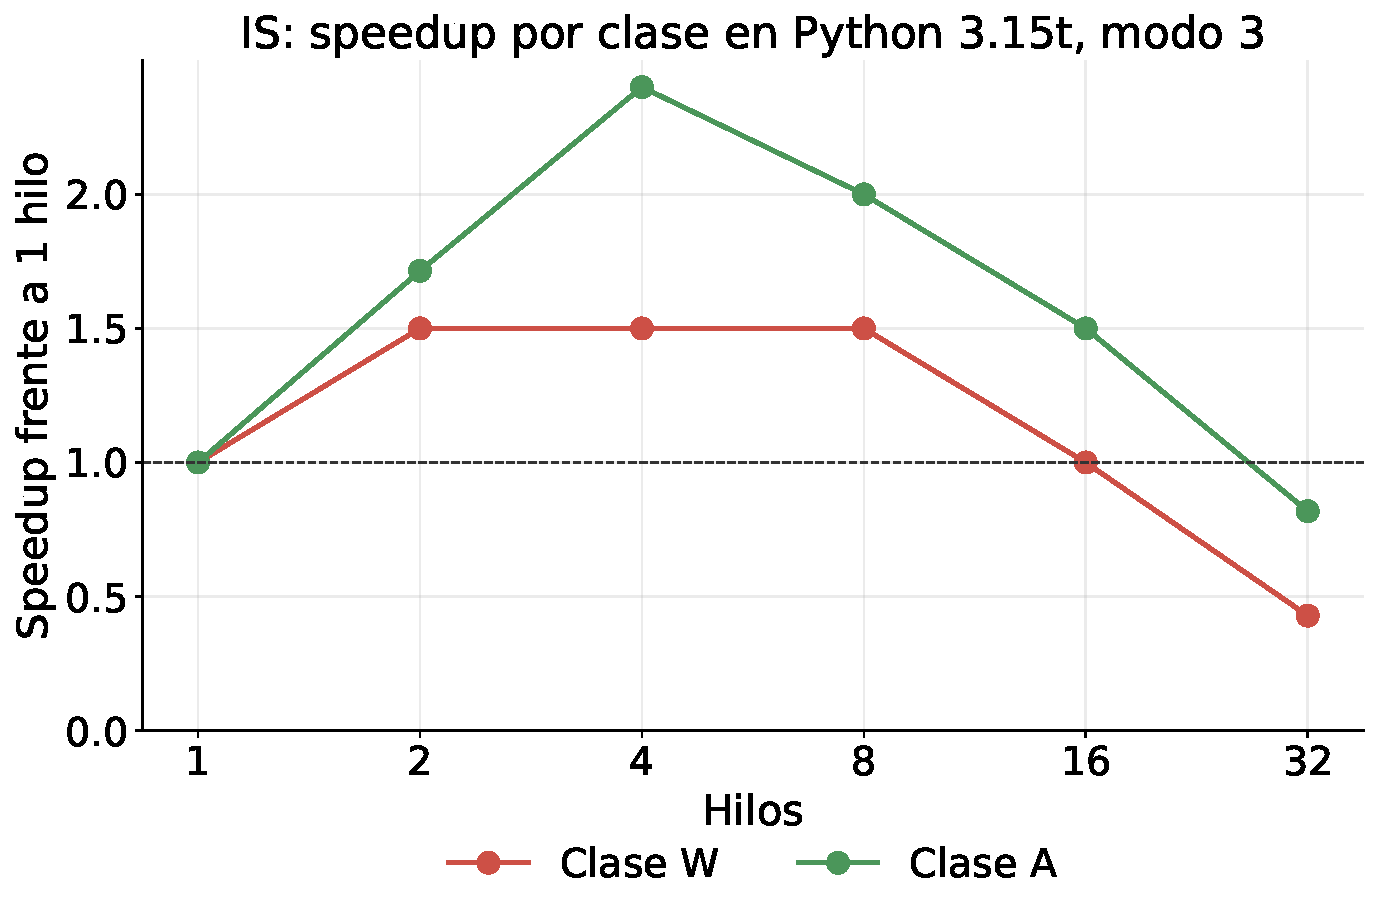
\includegraphics[width=\textwidth]{imagenes/resultados/benchmark_is_speedup_clases}
  \caption{IS.}
  \label{fig:resultados-is-clases}
\end{subfigure}

\vspace{0.8em}
\begin{subfigure}[t]{0.49\textwidth}
  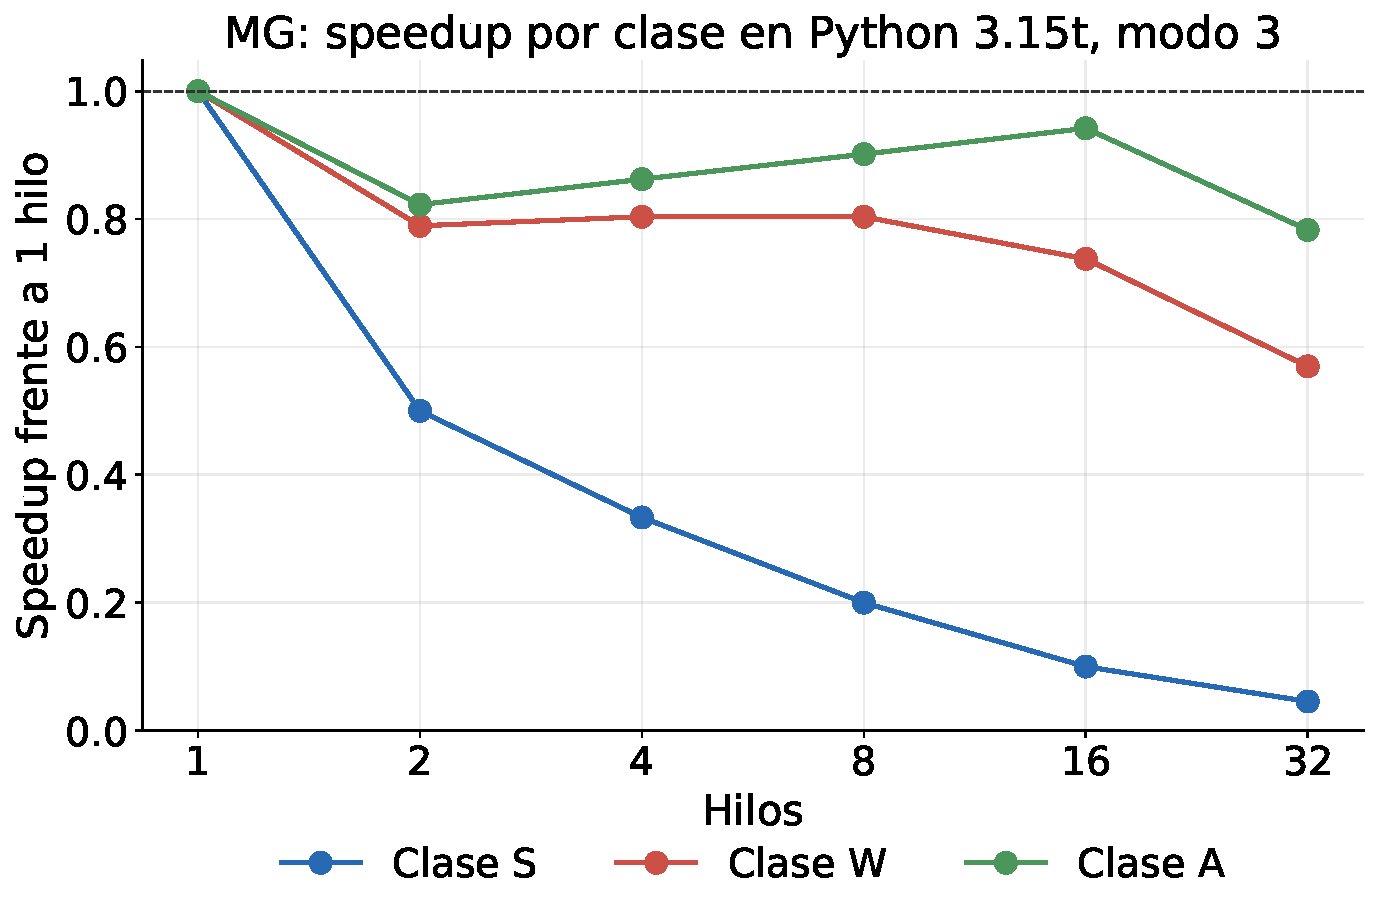
\includegraphics[width=\textwidth]{imagenes/resultados/benchmark_mg_speedup_clases}
  \caption{MG.}
  \label{fig:resultados-mg-clases}
\end{subfigure}
\caption{Speedup por clase (S, W, A) en modo~3, Python~3.15t, para cada
benchmark.}
\label{fig:resultados-benchmark-clases}
\end{figure}

La lectura por benchmark confirma la separación observada en las tablas. EP
mantiene una curva creciente en S, W y A. FT también mejora con el tamaño,
aunque su máximo aparece antes de 32~hilos. IS solo se beneficia de forma clara
en clase~A y con pocos hilos. CG y MG no mejoran al aumentar la clase. En este
punto, los resultados muestran el patrón, y el Capítulo~\ref{chap:profiling}
analiza sus causas mediante \texttt{perf stat}, muestreo y trazado de
Python~3.15.


\section{Limitaciones de la medida}
\label{sec:resultados-limitaciones}

Las amenazas transversales de la evaluación se recogen en la
Sección~\ref{sec:amenazas-validez}. En la campaña principal afectan sobre todo a
tres puntos. El primero es la resolución temporal de la salida NAS. Algunos
tiempos de clase~S, especialmente en IS y MG, aparecen como 0.00~s o 0.01~s.
Sirven para confirmar tiempos absolutos bajos, pero no para calcular ratios
finos.

El segundo es el uso del mejor tiempo de tres repeticiones como métrica principal
de rendimiento. La Sección~\ref{sec:tratamiento-resultados} contrasta esa
elección con mediana y rango, y muestra que la diferencia mediana entre la
mediana y el mejor tiempo queda por debajo del 0.5\% en las campañas compiladas y
se mantiene baja en los modos interpretados. No sustituye a una campaña
estadística más amplia, pero sí descarta que las conclusiones dependan de una
repetición aislada.

El tercero es que la clase~A solo se ejecutó en modo~3. No
hay medidas de modo~2 para A en la campaña final. La restricción fue
deliberada porque el modo~2 ya había demostrado tiempos demasiado altos en
clase~W. Las conclusiones de clase~A se refieren, pues, a la escalabilidad del
mejor modo disponible.


\section{Conclusiones del capítulo}
\label{sec:resultados-conclusiones}

La campaña principal deja un balance claro. Las cinco adaptaciones son
funcionalmente correctas en todos los caminos evaluados, y el modo~3 recorta de
forma decisiva los tiempos del modo~2. Con Python~3.15t, EP y FT escalan bien en
las clases mayores, pero esa escalabilidad no se generaliza a CG, IS y MG.

El Capítulo~\ref{chap:profiling} utiliza \texttt{perf stat} para relacionar
los speedups observados con ocupación real de CPU, IPC y eventos de memoria, y
el nuevo sistema de muestreo de Python~3.15 para atribuir el tiempo de
sincronización y el balance de carga por función e hilo. El
Capítulo~\ref{chap:versiones} compara estos resultados con Python~3.13t y
Python~3.14t.
